\section{导数}
在之前的笔记中,单调性可以描述一个函数在某一区间的增减性。但它具有局限性:我们只能知道一个大体的情况(增、减或非单调),而不能知道它的具体增减量为何。

再设想一下:我们通过描点法画出了函数上的几个点,要使用曲线连接把它们连接起来。由于两点之间的距离比较大,我们可能会画出几种不同的图像(如图\ref{fig:two-different-function-figure})。

\begin{figure}[htb]
    \centering
    \begin{tikzpicture}
        \draw[->] (-2, 0) -- (2, 0);
        \draw[->] (0, -2) -- (0, 2);
        \draw[color=blue,domain=-2:2] plot (\x, -0.55*\x*\x+0.15*\x+1.2);
		\filldraw (-1, 0.5) circle (1pt) (0, 1.2) circle (1pt) (1, 0.8) circle (1pt);
    \end{tikzpicture}
    \begin{tikzpicture}
        \draw[->] (-2, 0) -- (2, 0);
        \draw[->] (0, -2) -- (0, 2);
        \draw[color=orange,domain=-1.26346:1.2423] plot (\x, 2.1667*\x*\x*\x-0.55*\x*\x-2.01667*\x+1.2);
		\filldraw (-1, 0.5) circle (1pt) (0, 1.2) circle (1pt) (1, 0.8) circle (1pt);
    \end{tikzpicture}
    \caption{描点法作出的两种截然不同的图像}
    \label{fig:two-different-function-figure}
\end{figure}

当然,我们可以描更多的点作更精确的图像,那可就无穷无尽了。

不过如果我们知道一些更详细的函数性质,比如说函数只有一个递增区间和一个递减区间,那么就可以知道左图更符合目标函数的图像。

综上可以看出:过去研究的函数及其性质存在不足。故需要引入新的东西,叫做\textbf{导数}\footnote{“导数”即导函数,函数某一点处的斜率称为“导数值”。}。

求函数某一点导数值的公式如下\footnote{极限的求法不是重点,故不介绍。所以请自己领悟(笑)}:\[f'(x_0)=\lim_{h\rightarrow 0}\frac{f(x_0+h)-f(x_0)}{h}\]其几何意义是$y=f(x)$在点$(x_0, f(x_0))$处切线的斜率。

\begin{example}
	已知在使用某种杀菌剂$t$小时后室内细菌数量为$f(t)=10^5+10^4t-10^3t^2$

	\begin{enumlist}
		\item 求$f'(10)$的值
		\item 说出$f(10)$和$f'(10)$的实际意义
	\end{enumlist}
\end{example}
\begin{proof}[解小题1]
	根据公式可以得到:\[f'(10)=\lim_{h\rightarrow 0}\frac{f(10+h)-f(10)}{h}=-10000\qedhere\]
\end{proof}
\begin{proof}[解小题2]
	意义分别为:

	\begin{desclist}
	\item[$f(10)$] 在使用杀菌剂$10$小时后,室内细菌数量为$10000$个
	\item[$f'(10)$] 在使用杀菌剂$10$小时后,室内平均每小时减少$10000$个细菌
	\end{desclist}

	请注意实际意义和$f(x)$以及$f'(x)$意义的区别。
\end{proof}

知道了函数某一点处的斜率,我们就可以根据下面的公式:\[y-f(x_0)=f'(x_0)(x-x_0)\]求出该点的切线方程。

\begin{example}
	利用导数的定义求$y=x^2$在$x=1$处的导数$f'(1)$,并求此函数在$x=1$时的切线方程
\end{example}
\begin{proof}[解]
	先套公式得导数值:\[f'(1)=\lim_{h\rightarrow 0}\frac{(1+h)^2-1}{h}=\lim_{h\rightarrow 0}h+2=2\]

	然后求得切线方程:\[y-1=2(x-1)\Rightarrow y=2x-1\qedhere\]
\end{proof}

将求导数值的公式稍作修改,就可以得到导函数的定义求法:\[f'(x)=\lim_{h\rightarrow 0}\frac{f(x+h)-f(x)}{h}\]

\begin{example}
	用定义求$f(x)=x^2$的导函数
\end{example}
\begin{proof}[解]
	这道例题很简单,只需带入公式即可:\[f'(x)=\lim_{h\rightarrow 0}\frac{(x+h)^2-x^2}{h}=\lim_{h\rightarrow 0}2x+h=2x\qedhere\]
\end{proof}

\subsection{求导函数}
在上文,我们求出了$y=x^2$的导函数。使用定义求法当然可以求出很多函数的导函数。不过由于知识水平有限,更多函数的导函数是算不出来的,所以下面这个列表整理了基础函数的导函数:

\begin{desclist}
	\item[多项式函数] $(C)'=0$;$(x^a)'=ax^{a-1}$
	\item[指对函数] $(e^x)'=e^x$;$(\ln x)'=\frac{1}{x}$
	\item[三角函数] $(\sin x)'=\cos x$;$(\cos x)'=-\sin x$
\end{desclist}

此外,导数值为$0$的点称为函数的驻点。

\begin{example}
	求$y=\sin x$的导函数及其驻点
\end{example}
\begin{proof}[解]
	根据基础函数的导函数得:\[y'=(\sin x)'=\cos x\]

	解方程即可得驻点:\[\cos x=0\Rightarrow x=k\pi+\frac{\pi}{2}\qedhere\]
\end{proof}

我们知道初等数学有四则运算,那导数呢?肯定有四则运算,它的运算法则如下:

\begin{desclist}
	\item[加减法] $(f\pm g)'=f'\pm g'$
	\item[数乘] $(Cf)'=C\cdot f'$
	\item[乘法] $(f\cdot g)'=f'g+fg'$
	\item[除法] $(\frac{f}{g})'=\frac{f'g-fg'}{g^2}$
\end{desclist}

\begin{quote}
	如果不按照运算法则去计算导数,而仅仅凭错误的经验,老师说不定会生气到想要揍你哦(苦笑)
\end{quote}

咳咳,回到正题:注意四则运算中没有包括指数运算,不过这个是小事情,不用担心,过一会儿会介绍指数函数的求导。

\noindent\dotfill

要求对数函数的导数,要先利用换底公式:$\log_ax=\frac{\ln x}{\ln a}$,然后使用指对函数的求导公式求导:
\[(\log_ax)'=\frac{1}{x\ln a}\]

\begin{example}
	求$y=\log_2x$的导数
\end{example}
\begin{proof}[解]
	运用换底公式和导数的除法得:
	\[\begin{aligned}
		y'&=(\log_2x)'=(\frac{\ln x}{\ln2})' \\
		  &=(\frac{1}{\ln2}\cdot\ln x)'=\frac{1}{x\ln2}
	\end{aligned}\]

	注意$\frac{1}{\ln2}$是一个常数,可以提出。
\end{proof}

\noindent\dotfill

求三角函数的导数,需要全部化到一倍角后利用切割化弦,全部换成$\sin$和$\cos$后利用三角函数的求导公式求导。

其它三角函数的导函数:
\[
	\begin{aligned}
		(\tan x)'&=\sec^2x \\
		(\cot x)'&=-\csc^2x \\
		(\sec x)'&=\tan x\cdot\sec x \\
		(\csc x)'&=-\cot x\cdot\csc x
	\end{aligned}
\]

\begin{example}
	求$y=\sin2x$的导函数
\end{example}
\begin{proof}[解]
	依照上述求三角函数的导函数的方法可得:
	\[\begin{aligned}
		y'&=(\sin2x)'=2(\sin x\cos x)' \\
		  &=2[(\sin x)'\cos x+\sin x(\cos x)'] \\
		  &=2(\cos^2x-\sin^2x)=2\cos2x
	\end{aligned}\qedhere\]
\end{proof}

\subsubsection{复合函数的导数}
刚刚我们求过了$y=\sin2x$的导函数,这明显太麻烦了。对于这类可以复合的函数,我们可以使用下面的方法求导。

若$y=F(x)$可复合成$u=g(x)$和$y=f(u)$,那么$F'(x)=g'(x)f'(u)$,注意最后$u$要换回$x$。

\begin{example}
	求$y=\sin2x$的导函数
\end{example}
\begin{proof}[解]
	该函数可复合成如下函数:
	\[\begin{aligned}
		&u=2x \\
		&y=\sin u \\
	\end{aligned}\]

	则该函数的导函数为:\[y'=(2x)'(\sin u)'=2\cos u=2\cos 2x\qedhere\]
\end{proof}

利用对数恒等式得到$a^x=e^{\ln a^x}=e^{x\ln a}$,然后可利用复合函数求导得指数函数的导数(这里不设例题)。其公式为:\[(a^x)'=a^x\ln a\]

\begin{example}
	求$y=2^{2x+1}$的导函数
\end{example}
\begin{proof}[解]
	公式只能求$2^x$的导数,不能求$2^{2x+1}$,所以应该使用复合函数求导。

	该函数可复合成如下函数:
	\[\begin{aligned}
		&u=2x+1 \\
		&y=2^u \\
	\end{aligned}\]

	使用乘法公式得导函数:\[y'=(2x+1)'(2^u)'=2\ln 2\cdot2^u=2\ln2\cdot2^{2x+1}\qedhere\]
\end{proof}

\subsection{利用导函数研究函数性质}
导函数反应了原函数的增减情况,我们可以使用导函数间接研究函数性质。

上面提到过,驻点是导数值为$0$的点,在这个点上函数既不增也不减。以驻点为切入点研究函数性质正合适。

高中数学涉及的函数性质有:单调性、对称性、周期性以及最值值域。不过根据导数的性质,它可以求单调区间及最值值域。

\subsubsection{单调性}
导函数嘛,本来就是表示函数斜率的变化情况的,非常适合用来求单调性。

刚刚提过,在驻点上,函数不增也不减,我们就可以认为它是单调区间的临界值。不过这样的说法不是特别准确,可否恳请阁下仔细思考下面两个命题:

\begin{enumlist}
	\item 导函数无驻点,原函数是单调函数
	\item 导函数有驻点,原函数非单调
\end{enumlist}

命题$1$显然是真的,随便想想即可得出($y=x$)。对于命题$2$,我们可以观察$y=x^3$的图像及其导函数$y'=3x^2$的图像:$y=x^3$是严格增函数,继续观察导函数的图像可发现此函数有驻点$x=0$。故我们得出命题$2$是假命题。

根据导函数的几何意义,$f'(x)>0$的部分是单调递增区间;$f'(x)<0$的部分是单调递减区间(不建议解不等式,太麻烦)。

不过我们可以根据导函数求出驻点和无定义点,用驻点和无定义点将定义域分成若干部分,再判断每一部分导数值的符号从而确定该部分的单调性。驻点可以合并进单调区间。

\begin{example}
	求函数$y=x^3+x^2-x-1$的单调区间
\end{example}
\begin{proof}[解]
	先求导函数:\[y'=3x^2+2x-1\]

	再求驻点:\[3x^2+2x-1\Rightarrow x=-1\text{或}\frac{1}{3}\]

	驻点将定义域分成三段,求各段导数值的符号:
	\[\begin{aligned}
		(-\infty,-1]&\quad+ \\
		[-1, \frac{1}{3}]&\quad- \\
		[\frac{1}{3},+\infty)&\quad+
	\end{aligned}\]

	最后总结单调区间:
	\[\begin{aligned}
		\text{增区间:}&(-\infty,-1]\text{和}[\frac{1}{3},+\infty) \\
		\text{减区间:}&[-1,\frac{1}{3}]
	\end{aligned}\qedhere\]
\end{proof}

\subsubsection{极值点}
存在$x=x_1$附近的邻域($x_1$左边到$x_1$右边的一个很小的区间),使该区间内其它自变量对应的函数值都不大于$f(x_1)$,称$x_1$是函数的极大值点,$f(x_1)$是极大值。

根据上述的定义,求出的极大值点只是局部极大值,不是函数的最大值。观察图\ref{fig:figure-of-quartic-function},$B$处是局部极大值点,但$A$处才是函数的最值处。

\begin{figure}[htbp]
	\centering
	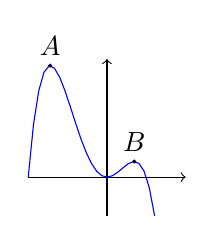
\begin{tikzpicture}[scale=0.5]
		\draw[->] (-2, 0) -- (2, 0);
		\draw[->] (0, -1) -- (0, 3);
		\draw[blue, domain=-2:1.21] plot(\x, -1 * \x * \x * \x * \x - \x * \x * \x + 2 * \x * \x);
		\filldraw (-1.443, 2.833) circle (1pt) node[above] {$A$};
		\filldraw (0.693, 0.397) circle (1pt) node[above] {$B$};
	\end{tikzpicture}
	\caption{$-x^4-x^3+2x^2$的图像}
	\label{fig:figure-of-quartic-function}
\end{figure}

和上面求单调区间一样,我们还是需要先求出导函数,然后求出驻点,再根据驻点附近$f'(x)$的符号判断此驻点是否为最值点。

\begin{example}
	求$y=\frac{1}{3}x^3-x+2$的极值点和极值
\end{example}
\begin{proof}[解]
	先求导函数得:\[y'=x^2-1\]

	解方程得驻点:\[x^2-1=0\Rightarrow x=\pm1\]

	计算各段的导数值可得增区间为$(-\infty,-1]\text{和}[1,+\infty)$,减区间$[-1,1]$,将驻点代入原函数即可得极大值。

	$\therefore$当$x=-1$时,有极大值$\frac{8}{3}$;当$x=1$时,有极大值$\frac{4}{3}$。
\end{proof}

\subsubsection{研究函数图像}\label{sec:mathsAnalysis-derivative-studyPorpertyOfFunction-figureOfFunction}
在上文,我们知道了如何用导函数求出原函数的单调区间以及极值点,这足以画出一个函数图像了(当然是不太精确的图像,不过关键的部分已经具备)。它常常用来求最值值域问题。

画函数图像嘛,也没啥技巧。端点和极值点描一下,无定义点处画渐近线,根据单调性把这些点连起来就是了。

\begin{example}
	用一张长宽都是$10$的正方形白纸,四周分别减去一块变长为$x$的正方形,折成一个简易垃圾桶,求该简易垃圾桶的最大容积
\end{example}
\begin{proof}[解]
	先列出容积$V$关于$x$的函数解析式,并标明定义域:\[V=x(10-2x)^2=4x^3-40x^2+100x(0<x<5)\]

	很显然,我们画不出它的图像,那么就应该使用导函数了:\[V'=12x^2-80x+100\]

	求出驻点:\[12x^2-80x+100=0\Rightarrow x=\frac{5}{3}\text{或}5\]

	这样定义域被分成$2$段:$[0,\frac{5}{3}]$和$[\frac{5}{3},5]$。通过计算各段的导数值可知函数在$[0,\frac{5}{3}]$上单调递增;在$[\frac{5}{3},5]$上单调递减。

	然后算出图像分别经过点$(0,0)$、$(\frac{5}{3},\frac{2000}{27})$和$(5,0)$,即可作出如图\ref{fig:drawing-figure-with-derivative}的函数图像,可得其最大值为$\frac{2000}{27}$。

	\begin{figure}[htbp]
		\centering
		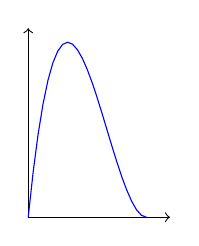
\begin{tikzpicture}[scale=0.3]
			\draw[->] (0, 0) -- (6, 0);
			\draw[->] (0, 0) -- (0, 8);
			\draw[blue,domain=0:5] plot(\x, 0.4 * \x * \x * \x - 4 * \x *\x + 10 * \x);
		\end{tikzpicture}
		\caption{通过导函数画出来的函数图像}
		\label{fig:drawing-figure-with-derivative}
	\end{figure}

	$\therefore$该简易垃圾桶的最大容积为$\frac{2000}{27}$。
\end{proof}

\begin{example}
	求$y=\frac{x^2-4x+12}{x-1}$在$x\in[0,+\infty)$的值域
\end{example}
